%!TEX encoding = UTF8
%!TEX root =notes.tex
\chapter{Fonctions : généralités}

Le but de ce chapitre est l'étude générale des fonctions réelles.
C'est le premier chapitre d'une série de $4$ chapitres sur les fonctions.
Les objectifs de cette année sont les suivants.
	\begin{enumerate}[label=$\bullet$]
		\item consolider la notion de fonction, comme exprimant la dépendance d'une variable par rapport à une autre ; 
		\item exploiter divers registres, notamment le registre algébrique et le registre graphique ;
		\item étendre la panoplie des fonctions de référence ;
		\item étudier les notions liées au variations et au extremums des fonctions.
	\end{enumerate}
Il s'agit ici de traiter les deux premiers points, c'est-à-dire la notion générale de fonction ainsi que quelques registres dans lesquels une fonction peut être traduite.

Les capacités visées à la fin du chapitres sont les suivantes.
	\begin{enumerate}
		\item Exploiter l'équation $y=f(x)$ d'une courbe : appartenance, calcul de coordonnées.
		\item Modéliser par des fonctions des situations issues des mathématiques, des autres disciplines.
		\item Résoudre une équation ou une inéquation du type $f(x)=k$, $f(x) < k$, en choisissant une méthode adaptée : graphique, algébrique, logicielle.
		%\item Résoudre une équation du type $f(x)=k$ en choisissant une méthode adaptée : graphique, algébrique, logicielle.
		\item Résoudre, graphiquement ou à l'aide d'un outil numérique, une équation ou inéquation du type $f(x)=g(x)$, $f(x) < g(x)$.
		%\item Résoudre, graphiquement ou à l'aide d'un outil numérique, une équation du type $f(x)=g(x)$.
	\end{enumerate}

	\section{Introduction}
	
	\dfn{Fonction, variable, constante}{
		On dit qu'une quantité $y\in\R$ s'exprime en \emph{fonction} d'une quantité $x\in\R$ lorsque, à chaque nombre $x$ possible, on peut associer \underline{une seule} valeur $y$.
		
		On note alors $x \mapsto y$ et $x$ est appelé la \emph{variable}.
		
		Si une quantité ne dépend pas de $x$, on l'appelle \emph{constante} ou \emph{indépendante} de $x$.
	}{}
	
	\nt{
		Pour faire signifier la dépendance de $y$ comme fonction de $x$, on utilise la notation fonctionnelle $y(x)$, lu \og $y$ de $x$ \fg.
		Ainsi, lorsque $x$ vaut $2$, la valeur associée sera $y(2)$, lu \og $y$ de $2$ \fg.
		
		Ceci permet de différencier les valeurs qui émanent de différents $x\in\R$ : $y(1), y(-3), y(\frac34), \dots$.
		
		La notation $y(x)$ est remplacée par $f(x)$ ($f$ pour fonction) pour se libérer la lettre $y$.
	}
	
	\ex{}{
		Le périmètre d'un cercle de rayon $R$ est donné par $2\pi \cdot R$.
		Un rayon détermine donc un unique périmètre, et la fonction périmètre, dépendant de la variable rayon, est donnée par
			\[ R\mapsto 2\pi\cdot R. \]
		En appelant $P$ cette fonction, on peut aussi noter 
			\[ P(R) = 2\pi \cdot R. \]	
	}{}
	
	\exe{}{
		\begin{enumerate}
			\item
			Montrer que le rayon d'un cercle est fonction de son périmètre et écrire la fonction associée.
			\item
			Montrer que l'aire d'un cercle est fonction de son rayon et écrire la fonction associée.
			\item
			En déduire que l'aire d'un cercle est fonction de son périmètre et écrire la fonction associée.
		\end{enumerate}
	}{}
	
	\exe{}{
		Un étudiant jette une balle dans les airs et mesure la hauteur de la balle tous les quarts de seconde.
		Il note ses résultats dans le tableau ci-dessous.
		\begin{center}
			\begin{tabular}{|c|c|c|c|c|c|c|c|}\hline
				Hauteur (cm) & 85 & 145 & 190 & 145 & 85 & 40 & 0 \\ \hline
				Temps (s) & 0 & 0,25 & 0,5 & 0,75 & 1 & 1,25 & 1,5 \\\hline
			\end{tabular}
		\end{center}
		
		\begin{enumerate}
			\item La hauteur est-elle une fonction du temps ? Justifier.
			\item Le temps est-il une fonction du temps ? Justifier.
		\end{enumerate}
	}{}
	
	\dfn{Fonction réelle, domaine}{
		Soit $\D \subset \R$ un ensemble de nombres qu'on appelle \emph{domaine}.
		
		Une fonction $f$ de $\D$ dans $\R$ associe à chaque élément $x\in\D$ du domaine un nombre $f(x) \in \R$.
		
		On note alors
			\begin{align*}
				f: \D & \longrightarrow \R \\
				x& \longmapsto f(x).
			\end{align*}
		
		\begin{center}
		    \begin{tikzpicture}[scale=1.2]
		        % domaine
		    	\coordinate (B) at (0,1);
		    	\coordinate (C) at (.1,.9);
		
		    	\node[dot=red, label=above:$x$] at (C){};
		    	
		    	\node[ellipse, draw, label=above:$\D \subset \R$, minimum height=110pt, minimum width=80pt] at (B){};
		
		        % codomaine
		    	\coordinate (D) at (4,.7);
		    	\node[dot=red, label=below:$f(x)$] at (D){};
		    	\node[ellipse, draw, label=above:$\R$, minimum height=60pt, minimum width=80pt] at (4,1){};
		
			%maps
			
		    	\draw[thick, ->] (C) -- (3.9,.72);
		    	\draw[thick, ->] (.6,1.5) -- (4,1.32);
		    	\draw[thick, ->] (.2,-.1) -- (4,1.18);
		    	
		    	% morepoitns
		    	
		    	\node[dot=black] at (0, 2){};		    	
		    	\node[dot=black] at (.2,-.1){};
		    	\node[dot=black] at (.6,1.5){};
		    	\node[dot=black] at (.75,.75){};
		    	\node[dot=black] at (-.3,1.4){};
		    	\node[dot=black] at (-.5,.2){};
		    	%\node[dot=black] at (.1,.9){};
		    	
		    	
		    	\node[dot=black] at (4.65,.75){};
		    	\node[dot=black] at (4.1,1.25){};
		    	\node[dot=black] at (4.6,1.35){};
		    	\node[dot=black]  at (3.45,.45){};
		    	%\node[dot=black]  at (4,.7){};
		    	\node[dot=black]  at (3.3,1.15){};
		
		    \end{tikzpicture}
		\end{center}
	}{}
	
	\ex{Fonctions vues en cours jusqu'ici}{
	
		\begin{enumerate}
			\item 
			La valeur absolue $|x|$ peut être formulée sous forme de fonction notée $|\cdot|$ : elle associe à chaque nombre réel sa valeur absolue.
			\begin{align*}
				|\cdot|: \R & \longrightarrow \R \\
				x& \longmapsto |x|.
			\end{align*}	
			
			\item
			Considérons la série statistiques $X_k$ suivante dépendant d'un entier naturel $k\in\N$.
				\begin{center}
				\begin{tabular}{|c|c|c|c|}\hline
					Valeur   & 0 & 20 & 10 \\ \hline
					Effectif & 17 & 17 & k \\ \hline
				\end{tabular}
				\end{center}
			La variance $\Var(X_k)$ est une fonction qui à tout entier naturel $k\in\N$ associe la variance de la série $X$.
			Au lieu de voir $\Var$ comme fonction de $X$, on la voir plutôt comme fonction de $k$.
			Nomons $f$ cette fonction pour ne pas utiliser surcharger la notation $\Var$.
			\begin{align}
			\begin{split}
				f: \N & \longrightarrow \R \\
				k& \longmapsto \Var(X_k)
			\end{split}\label{func:vark}
			\end{align}
			Remarquons que le domaine de $f$ est l'ensemble des entiers naturels $\N$.
			
			\item
			Pour définir l'écart type, il a fallu utiliser la fonction racine carrée.
			Comme la racine carrée d'un nombre négatif n'existe pas, le domaine de cette fonction est $[0;\pinfty[$, et non $\R$ tout entier.
				\begin{align*}
				\sqrt{\cdot}: [0;\pinfty[ & \longrightarrow \R \\
				x& \longmapsto \sqrt{x}
				\end{align*}

			\item 
			Une constante est en particulier une fonction d'une variable $x\in\R$ réelle.
			Ainsi la fonction $g$ donnée par
				\begin{align*}
				g: \R & \longrightarrow \R \\
				x& \longmapsto 42
				\end{align*}
			vaut constamment $42$, peut importe la valeur de $x$. 
			
			On voit dans l'expression $g(x) = 42$ que l'image de $x$ ne dépend aucunement de la valeur de $x$ :
			$g$ est une fonction constante.
						
		\end{enumerate}
	
	}{ex:fonctions-deja-vues}
	
	\dfn{Antécédent, image}{
		Considérons une fonction $f$ et deux nombres réels $x,y\in\R$ vérifiants
			\[ y = f(x). \]
		On lit \og $y$ égal $f$ de $x$ \fg, et on dit alors que
			\begin{enumerate}
				\item
				$y$ est l'\emph{image} de $x$ par $f$ ; et
				\item
				$x$ est \underline{un} \emph{antécédent} de $y$ par $f$.
			\end{enumerate}
	}{}
	
	\nt{
		\begin{enumerate}
			\item 
			Chaque $x\in\D$, élément du domaine, a \underline{exactement une} image par $f$ qui est $f(x)$.
			\item
			Un nombre $y\in\R$ peut avoir \underline{un, aucun, ou même plusieurs} antécédents. C'est le cas par exemple de $y=-1$ pour la fonction valeur absolue $f(x) = |x|$.
		\end{enumerate}
	}
	
	\ex{}{
		Considérons la fonction valeur absolue.
		On peut l'appeler $f$ en posant $f(x) = |x|$ pour tout $x\in\R$.
		
		Calculons les images de $1; 4; -1; -0,31; \frac23 ; -\frac23;$ et $0$.
			\begin{multicols}{2}
			\begin{enumerate}
				\item $f(1) = 1$
				\item $f(-1) = 1$
				\item $f( -0,31) = 0,31$
				\item $f\left(\dfrac23\right) = \dfrac23$
				\item $f\left( -\dfrac23\right) = \dfrac23$
				\item $f(0) = 0$
			\end{enumerate}
			\end{multicols}
			
		On en déduit les propositions suivantes.
			\begin{enumerate}[label=$\bullet$]
				\item
				L'image de $1$ par $f$ est $1$.
				\item
				L'image de $-1$ par $f$ est $1$.
				\item
				$1$ et $-1$ sont donc deux antécédents de $1$ par $f$.
				\item
				Un antécédent de $0,31$ par $f$ est $-0,31$.
				\item
				Un antécédent de $\dfrac23$ par $f$ est $\dfrac23$.
				\item
				Un antécédent de $\dfrac23$ par $f$ est $-\dfrac23$.
				\item
				$0$ est l'image et un antécédent de $0$ par $f$. C'est d'ailleurs le seul antécédent.
			\end{enumerate}
	}{}
	
	\exe{}{
		Considérons la fonction $f$ donnée par
		\begin{align*}
			f: \R & \longrightarrow \R \\
			x& \longmapsto 3\cdot x+1.
		\end{align*}
		Autrement dit, $f(x) = 3\cdot x + 1$ pour tout $x\in\R$.
		
		\begin{enumerate}
			\item
			Calculer l'image de $0$, de $3,1$, de $\frac13$, de $-1$, de $-\frac23$.
			\item
			Donner un antécédent de $1$.
			\item
			Déterminer tous les antécédents de $4$.	
		\end{enumerate}
	}{}
	
	\dfn{Forme algébrique}{
		On appelle 
			\[ f(x) = 3\cdot x+1 \]
		la forme \emph{algébrique} de $f$.
		On lit dans ce cas \og $f$ de $x$ égal trois $x$ plus 1 \fg.
		
		C'est une forme entièrement générale qui permet de déduire l'image $f(x)$ à partir de n'importe quel réel $x\in\D$ du domaine de $f$.
	}{}
	
	\newpage %temp
		
	\begin{figure}[!htb]
		\begin{subfigure}[b]{.45\textwidth}
\begin{mintedbox}{python}
def f(x):
	y = 2*x-3
	return y

f1 = f(1)
f2 = f(-1/2)


print(f1, f2)
\end{mintedbox}
		\caption{Programme 1.}
		\label{python:1}
		\end{subfigure}
		\begin{subfigure}[b]{.45\textwidth}
\begin{mintedbox}{python}
def f(x):
	y = x*x + 1
	z = -2*x
	return y+z

f1 = f(4)
f2 = f(-2)

print(f1, f2)
\end{mintedbox}
		\caption{Programme 2.}
		\label{python:2}
		\end{subfigure}
		\caption{Deux fonctions implémentées en Python.}
		\label{python:1-2}
	\end{figure}
	
	\exe{}{
		Lire les deux programmes Python de la figure \ref{python:1-2}.
		Quelles valeurs impriment-t-ils ?
		
		Écrire la fonction $f(x)$ de chaque programme sous forme algébrique.
	}{}
	
	\exe{}{
		On reconsidère la fonction $f$ de l'exemple \ref{ex:fonctions-deja-vues} donnée en $\eqref{func:vark}$.
		Utiliser la formule \eqref{eq:var} de la variance pour donner une expression algébrique de $f(k)$ dépendant de $k\in\N$, entier naturel.
		
		Calculer $f(10), f(20), f(50), f(100)$ et comparer les variances obtenues.
	}{exe:vark}
	
	\nt{
		Suite à l'exercice \ref{exe:vark} ci-dessus, on dira alors qu'on a écrit la variance \emph{en fonction de}  l'entier naturel $k\in\N$.
		
		L'expression algébrique permet de calculer facilement plusieurs images sans refaire le raisonnement à chaque fois.
	}
	
	\exe{}{
		Un fonction $f$ admet le tableau de valeurs suivant.
			\begin{center}
			\begin{tabular}{|c|c|c|c|c|}\hline
				$x$ & 0 & -2 & 1 & -1 \\ \hline
				$f(x)$ & 1 & 0 & 0 & 1 \\ \hline
			\end{tabular}
			\end{center}
		Parmis les expressions algébriques suivantes, trouver celle qui correspond à $f(x)$.
			\begin{multicols}{2}
			\begin{enumerate}[label=\roman*)]
				\item $1-x$
				\item $1+\dfrac{x}2$
				\item $\dfrac{1-x}2$
				\item $\dfrac{-x^2 - x + 2}2$
			\end{enumerate}
			\end{multicols}
	}{}
	

	\section{Représentation graphique}
	
	On souhaite représenter graphiquement une fonction $f$ afin de pouvoir rapidement trouver plusieurs informations sur $f$.
	Une bonne représentation graphique nous permet de lire
		%\begin{multicols}{2}
		\begin{enumerate}[label=$\bullet$]
			\item les images $f(x)$;
			\item les antécédents $x$ ;
			\item les variations de $f$ (croissante, décroissante, constante) ;
			\item le signe de $f(x)$ (positif, négatif, nul).
		\end{enumerate}
		%\end{multicols}
	
	Pour chaque $x\in\D\subset\R$, élément du domaine de $f$, il faut donc pouvoir facilement lire son image $f(x)$ par $f$.
	À cette fin et pour chaque $x\in\D$, on crée un point d'abscisse $x$ et d'ordonnée $f(x)$.
	L'ensemble de ces points est la courbe représentative de $f$.
	Pour lire l'image de $x$ par $f$, il suffit alors de trouver l'ordonnée de l'unique point de la courbe d'abscisse $x$.
	
	\dfn{Courbe représentative}{
		Considérons $f : \D \rightarrow \R$ une fonction.
		
		La \emph{courbe représentative} de $f$, notée $\C_f$, est donnée par l'ensemble de points
			\[ \C_f = \left\{ \left(x ; f(x) \right) \text{ où } x\in\D \right\}. \]
		On lit \og la courbe représentative de $f$ est l'ensemble des points $(x,f(x))$ du plan où $x$ parcourt le domaine de $f$ \fg.
	}{}	
	
	\cor{Propriété fondamentale}{
		On a donc la propriété fondamentale suivante valable pour tout $x,y\in\R$.
			\begin{align*}
				(x;y) \in \C_f && \iff && y = f(x).
			\end{align*}
			
			
			\begin{center}
			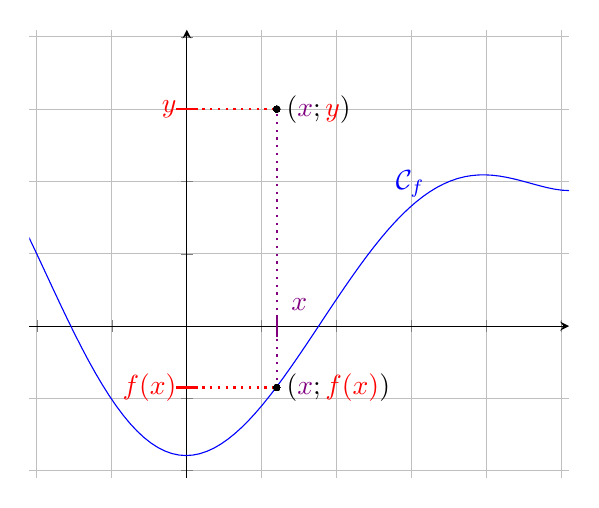
\begin{tikzpicture}[>=stealth]
				\begin{axis}[xmin = -2.1, xmax=5.1, xtick={-2, ..., 5},xticklabel=\empty, ymin=-2.1, ymax=4.1, ytick={-2, ...,4}, yticklabel=\empty, axis x line=middle, axis y line=middle, axis line style=->, grid=both]
					\addplot[no marks, blue, -] expression[domain=-4.1: 5.1, samples=100]{(x+3.5)*(x+2.5)*(x-3.5)*(x-4.5)*(x-5.5)/200 + 2}
					node[pos=.86, above]{$\mathcal{C}_f $};
					
					\addplot[black, mark=*, mark size = 1] (1.2,3) node[above, right] {$({\color{violet}x};{\color{red}y})$};
					\addplot[black, mark=*, mark size = 1] (1.2,-.85) node[below, right] {$({\color{violet}x};{\color{red}f(x)})$};
					
					\draw[violet, dotted, thick] (axis cs:1.2, -.85) -- (axis cs:1.2,3);
					\addplot[red, dotted, thick, domain = 0:1.2, samples=2] {3};
					\addplot[red, dotted, thick, domain = 0:1.2, samples=2] {-.85};
					
					\addplot[violet, thick, mark=|, mark size = 4] (1.2,0); % x cross
					\addplot[violet] (1.5,0) node[above=2pt] {$x$}; % x label
					\addplot[red, thick, mark=-, mark size = 4] (0,3) node[left] {$y$};
					\addplot[red, thick, mark=-, mark size = 4] (0,-.85) node[left] {$f(x)$};
				\end{axis}
			
			\end{tikzpicture}
			\end{center}
		Note : $f(x) = \dfrac1{200}(x+3,5)(x+2,5)(x-3,5)(x-4,5)(x-5,5) + 2$, polynôme de degré $5$ dans l'exemple ci-dessus.
	}{cor:prop-fond}
	
	\ex{}{
		Soit la fonction $f : [-1,5; 2,5] \rightarrow \R$ donnée algébriquement par
			\[ f(x) = 3\cdot x^3 -x - 3, \]
		et considérons les points $P(0;-3), Q(1; 1), R(-1; 1),$ et $S(2; 19)$.
		On se demande si les points appartiennent à la courbe représentative de $f$ ou non.
		
		D'après la propriété fondamentale \ref{cor:prop-fond}, un point $(x;y)$ appartient à la courbe de $f$ si et seulement si l'équation $y=f(x)$ est vérifiée.
		On a donc les (non) appartenances suivantes.
			\begin{enumerate}
				\item $f(0) = -3$, et donc $P \in \C_f$.
				\item $f(1) = -1 \neq 1$, donc $Q \not\in \C_f$.
				\item $f(-1) = -5 \neq 1$, donc $R \not\in\C_f$.
				\item $f(2) = 19$, et donc $S\in\C_f$.
			\end{enumerate}
		La courbe $\C_f$ est donnée ci-dessous.
			\begin{center}
			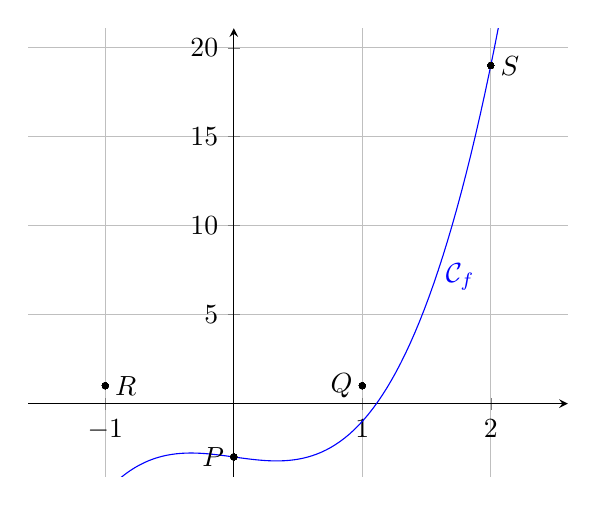
\begin{tikzpicture}[>=stealth]
				\begin{axis}[xmin = -1.6, xmax=2.6, ymin=-4.1, ymax=21.1, axis x line=middle, axis y line=middle, axis line style=->, grid=both]
					\addplot[no marks, blue, -] expression[domain=-1.1: 2.5, samples=100]{3*x^3 -x -3}
					node[pos=.3, right]{$\mathcal{C}_f$};
					
					\addplot[black, mark=*, mark size = 1] (0,-3) node[left] {$P$};
					\addplot[black, mark=*, mark size = 1] (1,1) node[below, left] {$Q$};
					\addplot[black, mark=*, mark size = 1] (-1,1) node[below, right] {$R$};
					\addplot[black, mark=*, mark size = 1] (2,19) node[below, right] {$S$};
				\end{axis}
			
			\end{tikzpicture}
			\end{center}
	}{}
	
	
	\exe{}{
		Considérons la fonction $f: \left]{-}\dfrac72 ; \dfrac{11}2 \right[ \rightarrow\R$ donnée algébriquement par
			\[ f(x) = \dfrac17-x. \]
		Pour chaque point suivant, déterminer s'il appartient à $\C_f$ ou non.
		
		\begin{multicols}{2}
		\begin{enumerate}[label=\roman*)]
			\item $\left(0; \dfrac17\right)$
			\item $\left(\dfrac17 ; 0\right)$
			\item $\left(\dfrac27 ; \dfrac37\right)$
			\item $\left(-\dfrac{13}7 ; 2\right)$
			\item $\left(\dfrac67 ; 1\right)$
			\item $\left(\dfrac27 ; -\dfrac17\right)$
		\end{enumerate}
		\end{multicols}
	
	}{}
	
	\exe{}{
		Considérons deux fonctions $f, g: ]{-}3 ; 3[ \rightarrow\R$ données algébriquement par
			\begin{align*}
				f(x) = x^2 - 2\cdot x && g(x) = (x-1)^2
			\end{align*}
		
		\begin{enumerate}
			\item Esquisser les représentations graphiques de $f$ et de $g$ dans un même repère.
			\item Démontrer que $g(x) - 1 = f(x)$ pour tout $x$ du domaine.
			\item En déduire que $(x-1)^2 = x^2 - 2\cdot x + 1$.
		\end{enumerate}
	}{}
	
	\exe{}{
		Esquisser la courbe de la fonction $f:[-2; 4]\rightarrow\R$ donnée algébriquement par
			\[ f(x) = 3. \]
		Que dire de $f$ et de $\C_f$ ?
	}{}
	
	\exe{}{
		Considérons la représentation graphique suivante d'une fonction $f$ définie sur $\D = ]{-}3,4 ; 2,3[$.
		
			\begin{center}
			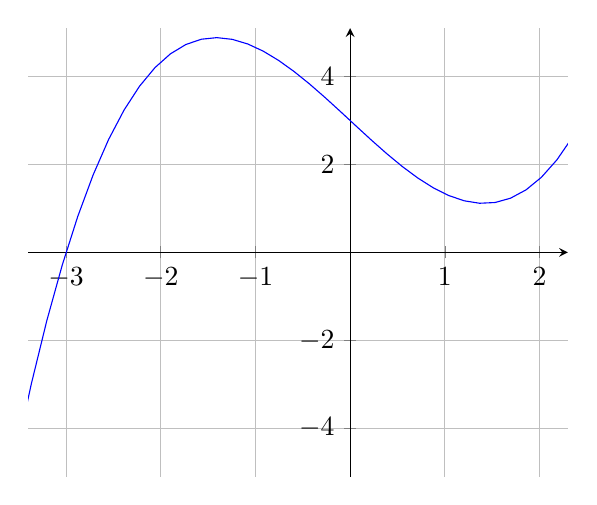
\begin{tikzpicture}[>=stealth]
				\begin{axis}[xmin = -3.4, xmax=2.3, ymin=-5.1, ymax=5.1, axis x line=middle, axis y line=middle, axis line style=->, grid=both]
					\addplot[no marks, blue, -] expression[domain=-5:3, samples=50]{x^3 /3 - 2*x +3}
					node[pos=.3, right]{$\mathcal{C}_f$};
				\end{axis}
			\end{tikzpicture}
			\end{center}
		\begin{enumerate}
			\item Donner approximativement les images de $-1,5$ et de $\dfrac{20}7$ par $f$.
			\item Énumérer approximativement les antécédents de $-2$ et de $2$ par $f$.
			\item Donner approximativement un réel qui admet exactement deux antécédents par $f$.
			\item Si $f$ était définie sur $\R$ tout entier, serait-il toujours possible de connaître l'image de $-2$ ? Et tous les antécédents de $-2$ ?
		\end{enumerate}
		Supposons désormais que $f(x) = 3-2\cdot x +\dfrac13 \cdot x^3$ pour tout $x\in\D$ du domaine.
		\begin{enumerate}
			\item[5.] Vérifier à la calculatrice les réponses aux deux premières questions.
			\item[6.] Montrer sans calculatrice que l'image par $f$ de $-3$ est $0$ et que l'image par $f$ de $0$ est $3$.
		\end{enumerate}
	}{}
	
	
	\exe{}{
		Un fonction $f$ admet une représentation graphique suivante.
			\begin{center}
			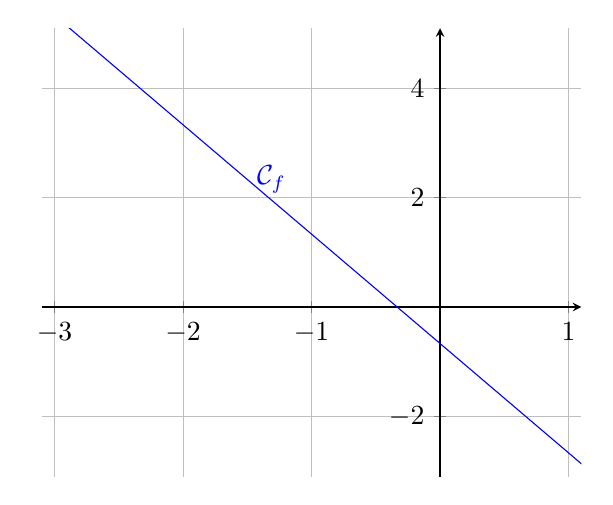
\begin{tikzpicture}[>=stealth]
				\begin{axis}[xmin = -3.1, xmax=1.1, ymin=-3.1, ymax=5.1, axis x line=middle, axis y line=middle, axis line style=->, grid=both]
					\addplot[no marks, blue, -] expression[domain=-3:2, samples=2]{-2/3 - 2*x}
					node[pos=.3, right]{$\mathcal{C}_f$};
				\end{axis}
			
			\end{tikzpicture}
			\end{center}
		Parmis les expressions algébriques suivantes, trouver celle qui correspond à $f(x)$.
			\begin{multicols}{2}
			\begin{enumerate}[label=\roman*)]
				\item $1-x$
				\item $\dfrac{-1-x}3$
				\item $\left(x+\dfrac13\right)^2$
				\item $-2\cdot x - \dfrac23$
			\end{enumerate}
			\end{multicols}
	}{}
	
	\section{Résolutions graphiques d'équations et d'inéquations}
	
	Le but de cette partie est d'étudier graphiquement les solutions, c'est-à-dire l'ensemble des nombres réels $x$ appartenant au domaine $\D$ commun à deux fonctions $f, g$ et vérifiant des (in)équations du type
		\begin{multicols}{2}
		\begin{enumerate}[label=$\bullet$]
			\item $f(x) = k$
			\item $f(x) < k$
			\item $f(x) = g(x)$
			\item $f(x) < g(x)$
		\end{enumerate}
		\end{multicols}
	\noindent où $k\in\R$ est un réel quelconque.